\documentclass[11pt]{article}
\usepackage{graphicx}
\usepackage{float}
\usepackage{amsmath}
\usepackage{amsfonts}
\usepackage[brazilian]{babel}
\usepackage[utf8]{inputenc}
\usepackage[T1]{fontenc}

\begin{document}

\title{Funções do Segundo Grau}
\author{Erik Perillo}
\date{}
\maketitle
\begin{abstract}
Nesta etapa, vamos falar do passo natural após as funções do primeiro grau.
\end{abstract}

\newpage

\tableofcontents

\newpage

\section{Formato da expressão}
\paragraph{}
A função do segundo grau, ou função quadrática,
é apenas uma extensão da função do primeiro grau.
Lembrando que, no caso da função do primeiro grau, tínhamos:
$$f(x) = a + bx$$
Vamos agora adicionar um novo termo à expressão e obter:
$$f(x) = a + bx + cx^2$$
Viu a diferença? Apenas adicionamos um novo $x$, agora elevado ao quadrado, 
junto com um termo multiplicativo. Esse é o formato geral de uma função 
quadrática.

\section{A cara da função}
Como fica a cara dessa função? Vamos primeiro analisar um caso em que 
$a$ e $b$ são nulos. Assim, temos:
$$f(x) = cx^2$$
Vamos pegar um exemplo para o valor $c$, digamos, $3$. Temos, assim, 
$f(x) = 3x^2$. Vamos pegar alguns valores de $x$ e construir uma tabela:
\newline
\begin{table}[H]
	\centering
	\begin{tabular}{| c | c |}
		\hline
		x & $f(x) = 3x^2$\\
		\hline
		0 & 0\\
		\hline
		1 & 3\\
		\hline
		2 & 12\\
		\hline
		3 & 27\\
		\hline
		4 & 48\\
		\hline
		5 & 75\\
		\hline
	\end{tabular}
\end{table}
\paragraph{}
Se colocarmos esses pontos no plano cartesiano, 
vamos obter:
\begin{figure}[H]
	\centering
	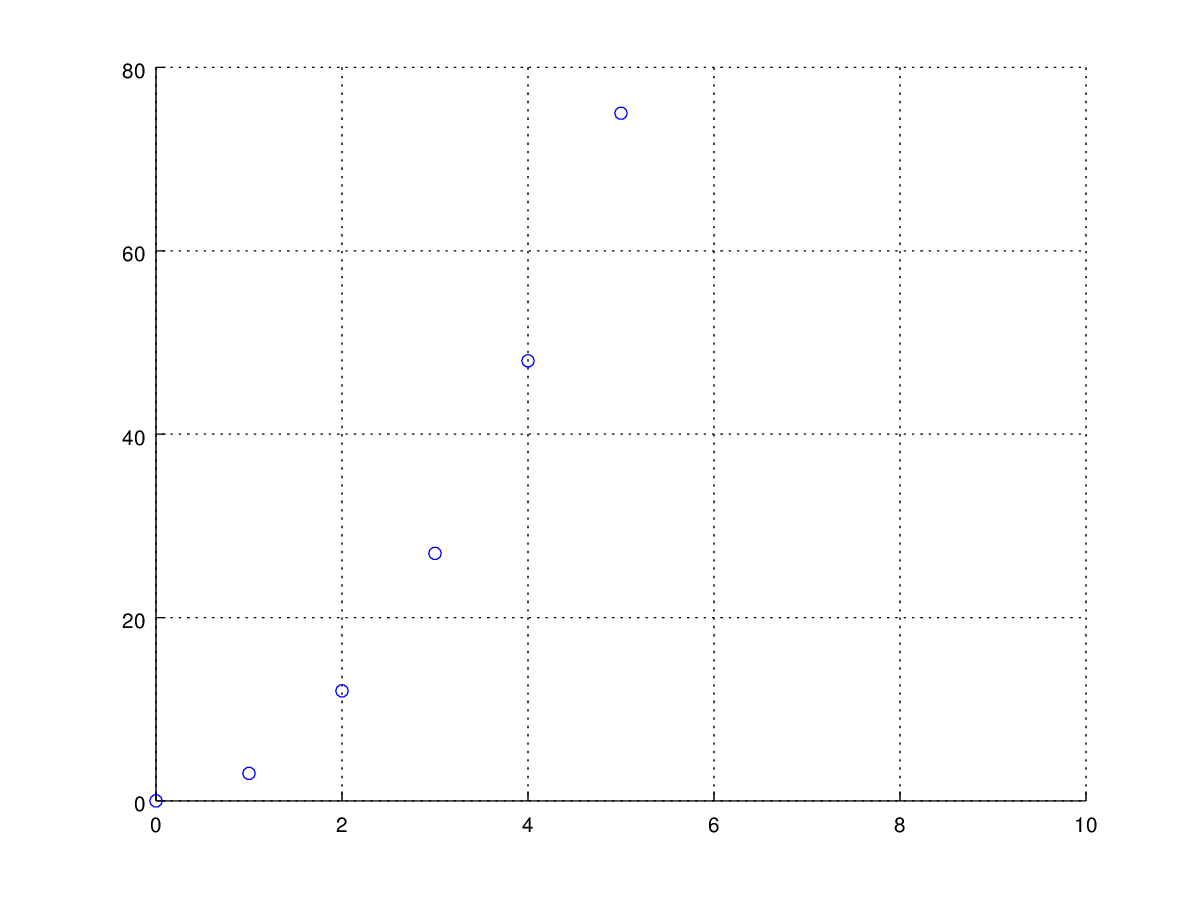
\includegraphics[width=0.8\linewidth]{imgs2/chart1.png}
\end{figure}
Veja como ela cresce rápido! Ela cresce desse jeito porque o $x$ está 
multiplicando por ele mesmo. Assim, quanto maior ele fica, maior fica o
produto dele por ele mesmo. Se fizermos isso em todos os pontos, vamos
obter:
\begin{figure}[H]
	\centering
	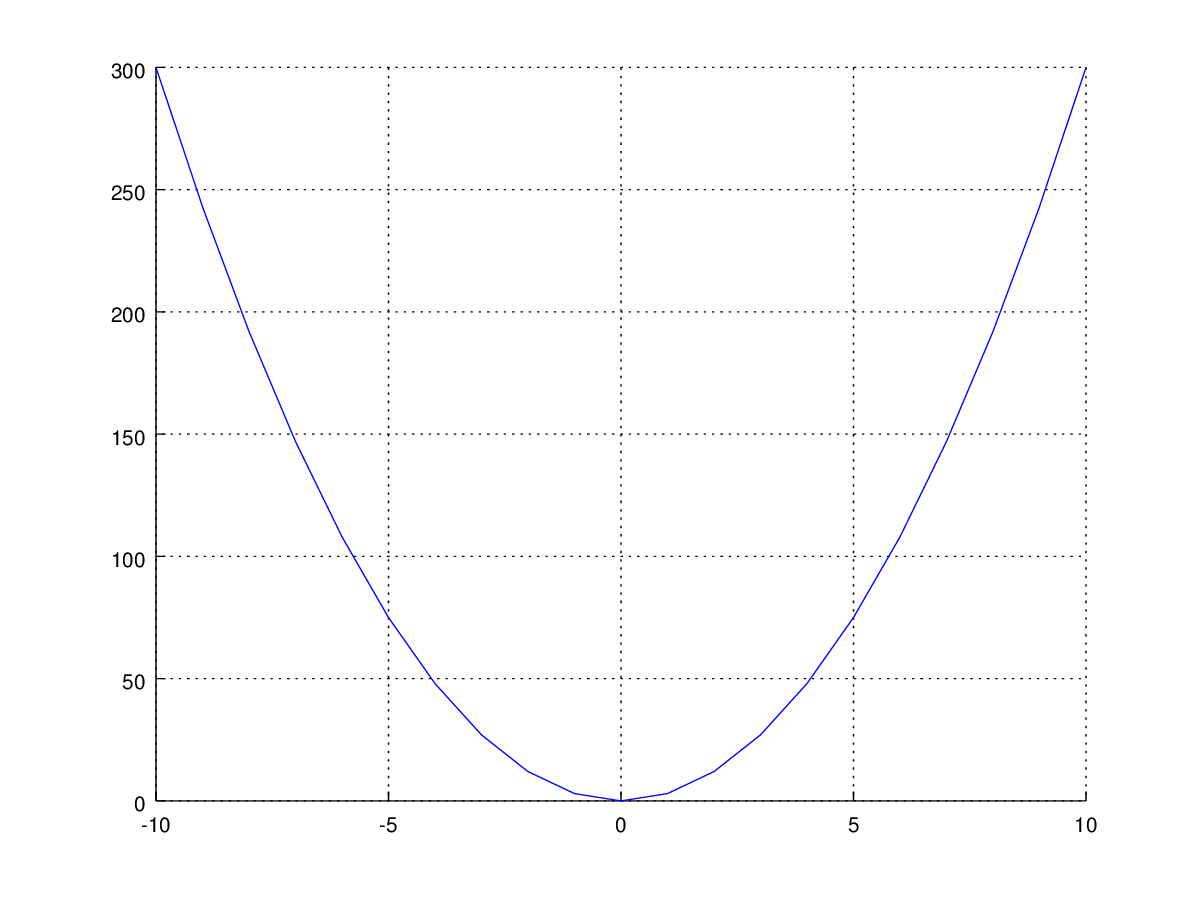
\includegraphics[width=0.8\linewidth]{imgs2/chart2.png}
\end{figure}
Estranho, não? Primeiro foque na parte onde x é positivo. Nesse caso, é
muito parecido com os pontos da figura anterior. Quanto x é negativo, o 
valor da função é exatamente o mesmo do valor com o x positivo, porque,
para qualquer número a, ${(a)}^2 = {(-a)}^2$! 
\paragraph{}
A função quadrática é sempre \textbf{simétrica}. Ao formato dela, damos
o nome de \textbf{parábola}.

\subsection{Concavidade}
\paragraph{}
Como o $x^2$ sempre vai ser maior que todo mundo uma hora, é o termo que 
acompanha ele (c) que manda. Assim, se c for negativo, a função vai ser
negativa uma hora ou outra. Se for positivo, vai ser positiva.
\paragraph{}
No caso em que c é positivo, dizemos que a função tem 
\textit{concavidade para cima}:
\begin{figure}[H]
	\centering
	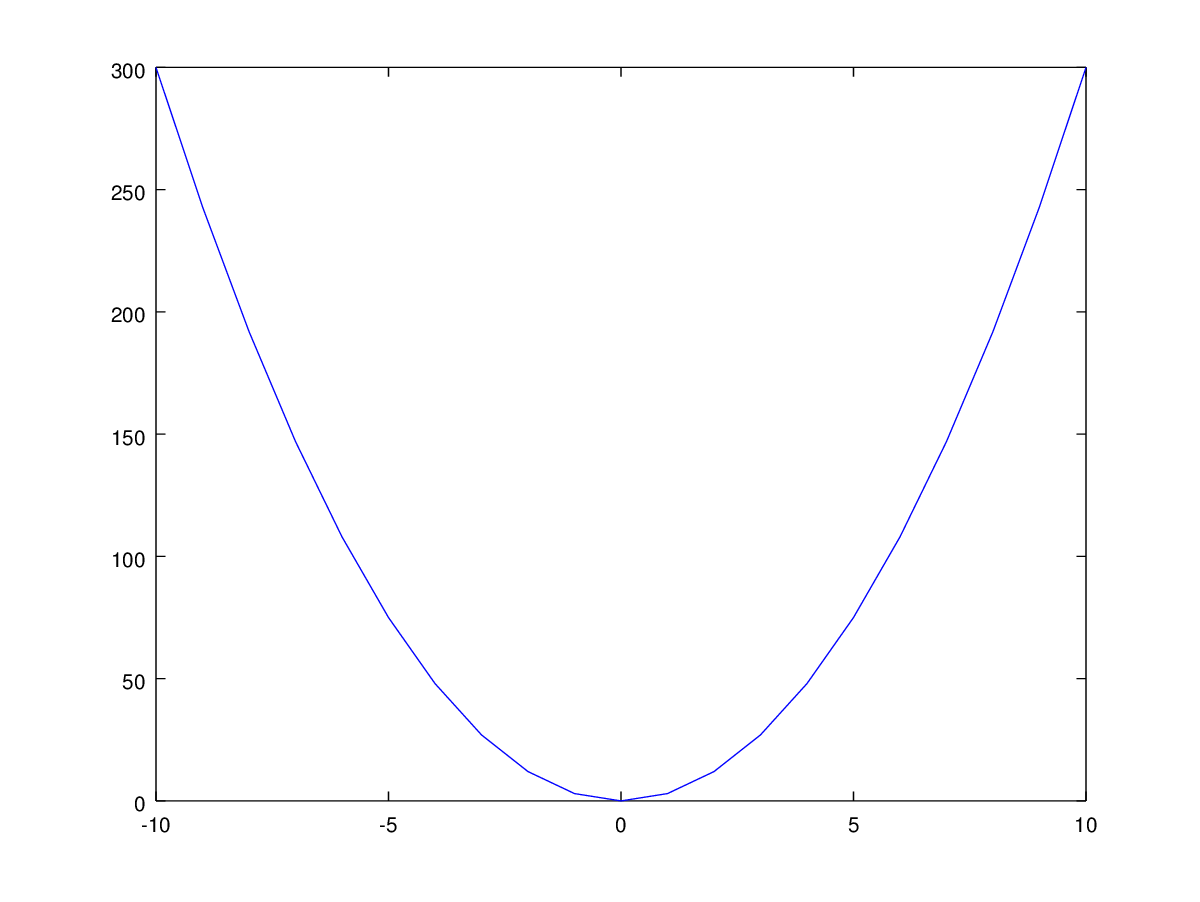
\includegraphics[width=0.8\linewidth]{imgs2/chart3.png}
	\caption{Um exemplo de concavidade para cima}
\end{figure}
No caso em que é negativo, dizemos que ela tem \textit{concavidade para 
baixo}:
\begin{figure}[H]
	\centering
	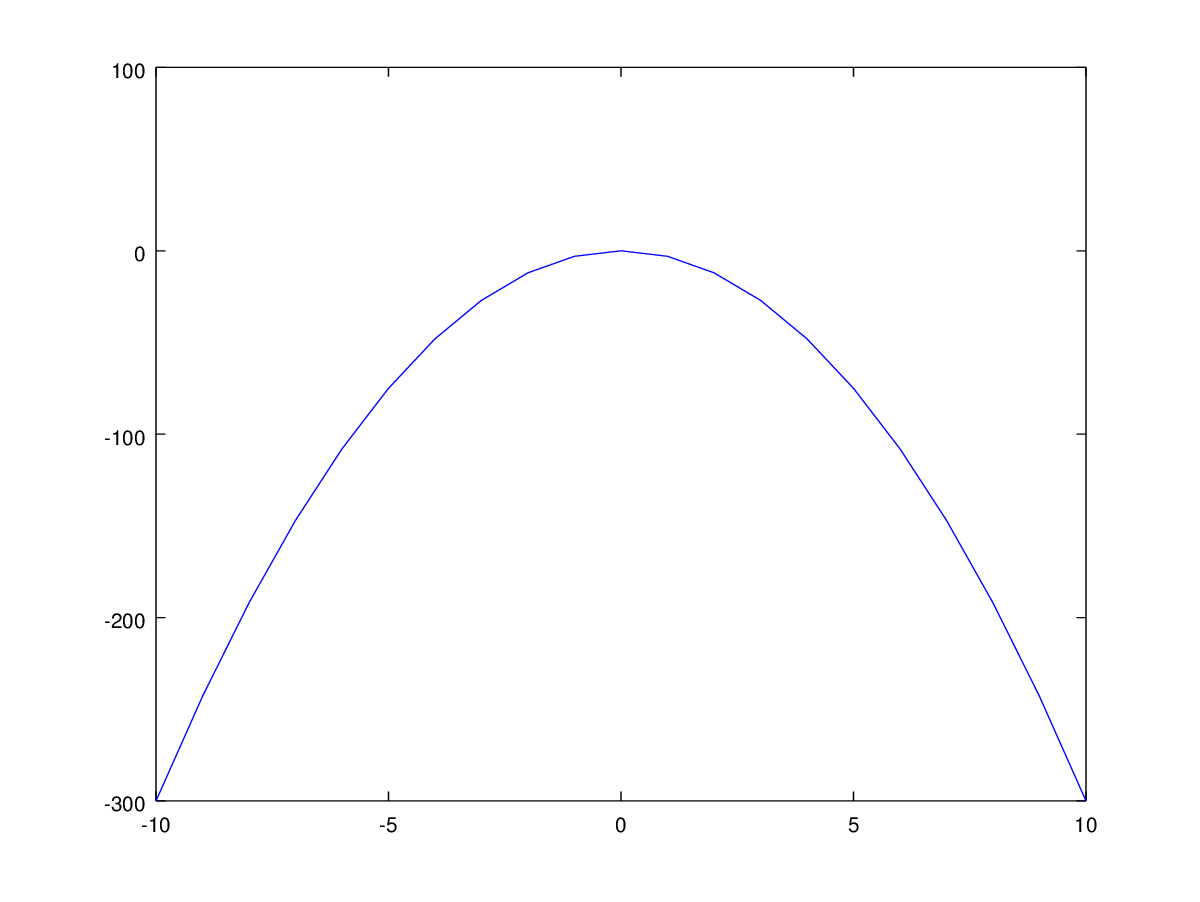
\includegraphics[width=0.8\linewidth]{imgs2/chart4.png}
	\caption{Um exemplo de concavidade para baixo}
\end{figure}

\subsection{Cruzada com o eixo y}
\paragraph{}
Como no caso da função do primeiro grau, a função cruza no eixo $y$ quando
$x = 0$ e então no termo $a$.

\section{Raízes da função}
\paragraph{}
Essa parte tem decoreba e não há o que fazer.
Para determinar as raizes da função linear, era muito fácil, bastava
isolar o $x$. Isso não é possível para a equação do segundo grau. 
Para funções do segundo grau, ou você tem uma raiz, ou tem duas, ou tem 
nenhuma. Dizemos então que você tem as soluções $x_1$ e $x_2$.
\paragraph{}
Para se resolver as raízes, usamos a fórmula de \textit{Bhaskara}:
$$\Delta = \sqrt{b^2 - 4ac}$$
Chamamos esse símbolo ($\Delta$) de \emph{delta}.
Temos, então, que:
$$x = \frac{-b \pm \sqrt{\Delta}}{2a}$$
\newpage
Temos três casos para delta:
\begin{itemize}
	\item Quando $\Delta$ é positivo, temos duas raízes diferentes, ou seja,
		\textbf{a função cruza pelo eixo x duas vezes}.
	\item Quando $\Delta$ é zero, temos duas raízes iguais, ou seja,
		\textbf{a função cruza pelo eixo x apenas uma vez}.
	\item Quando $\Delta$ é negativo, não temos $x \in \mathbb{R}$, ou seja,
		\textbf{a função não cruza pelo eixo x nenhuma vez}.
\end{itemize}

\begin{figure}[H]
	\centering
	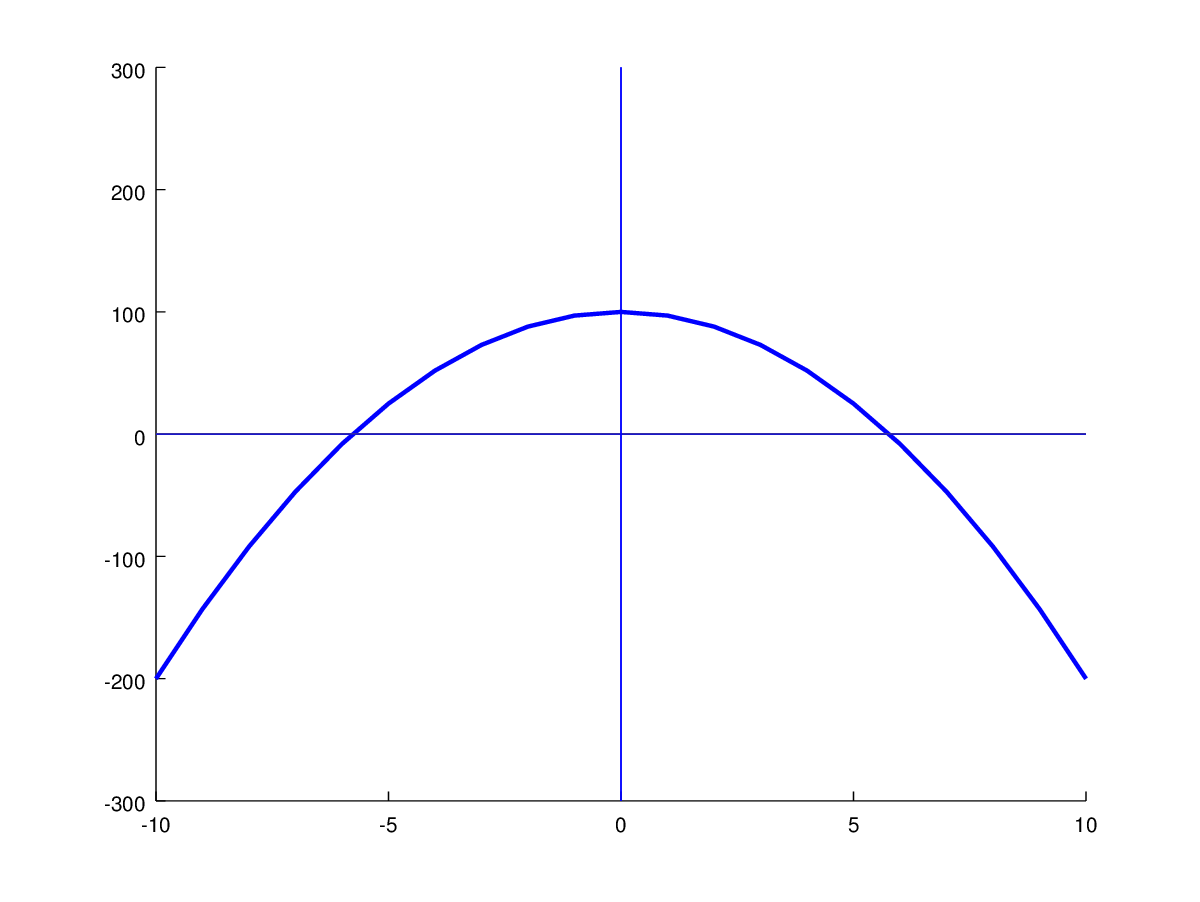
\includegraphics[width=0.8\linewidth]{imgs2/chart5.png}
	\caption{Um exemplo de $\Delta > 0$}
\end{figure}

\begin{figure}[H]
	\centering
	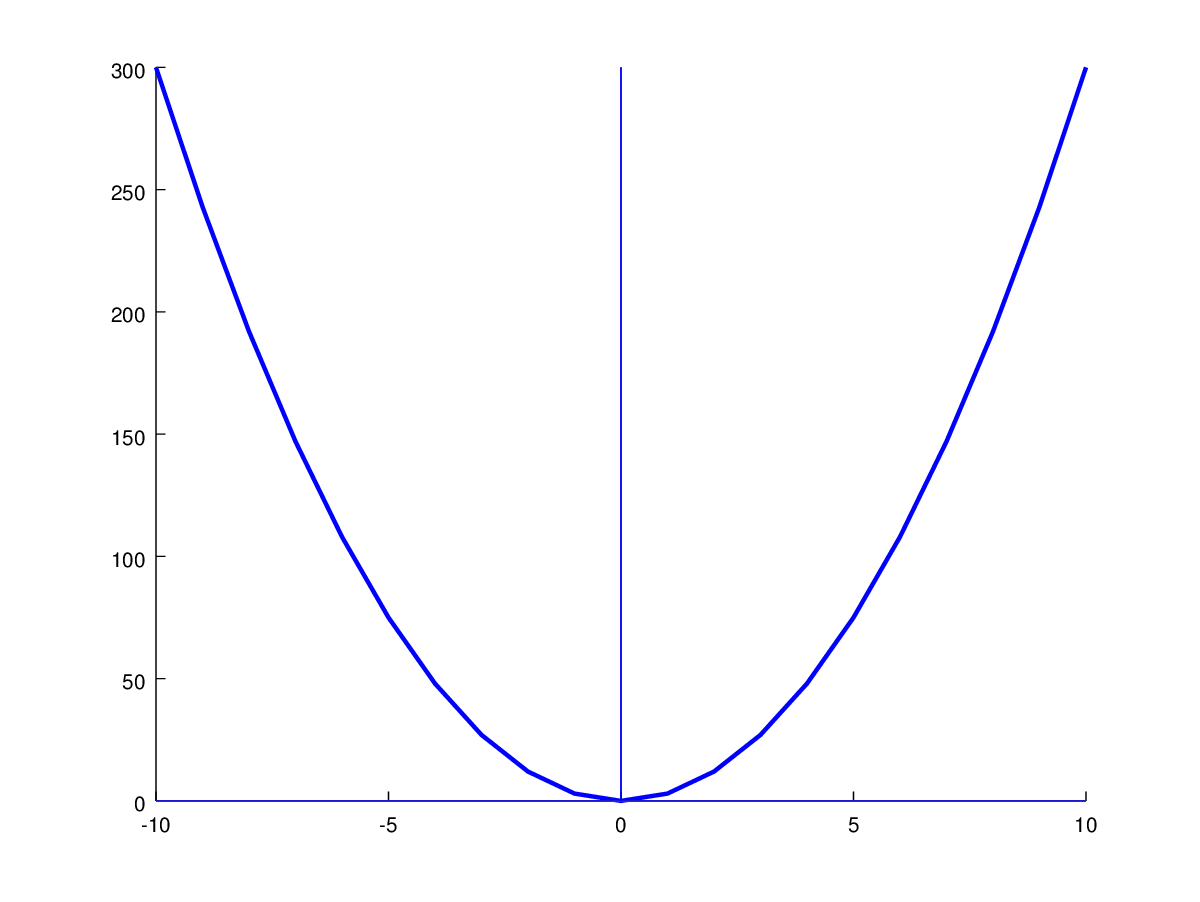
\includegraphics[width=0.8\linewidth]{imgs2/chart6.png}
	\caption{Um exemplo de $\Delta = 0$}
\end{figure}

\begin{figure}[H]
	\centering
	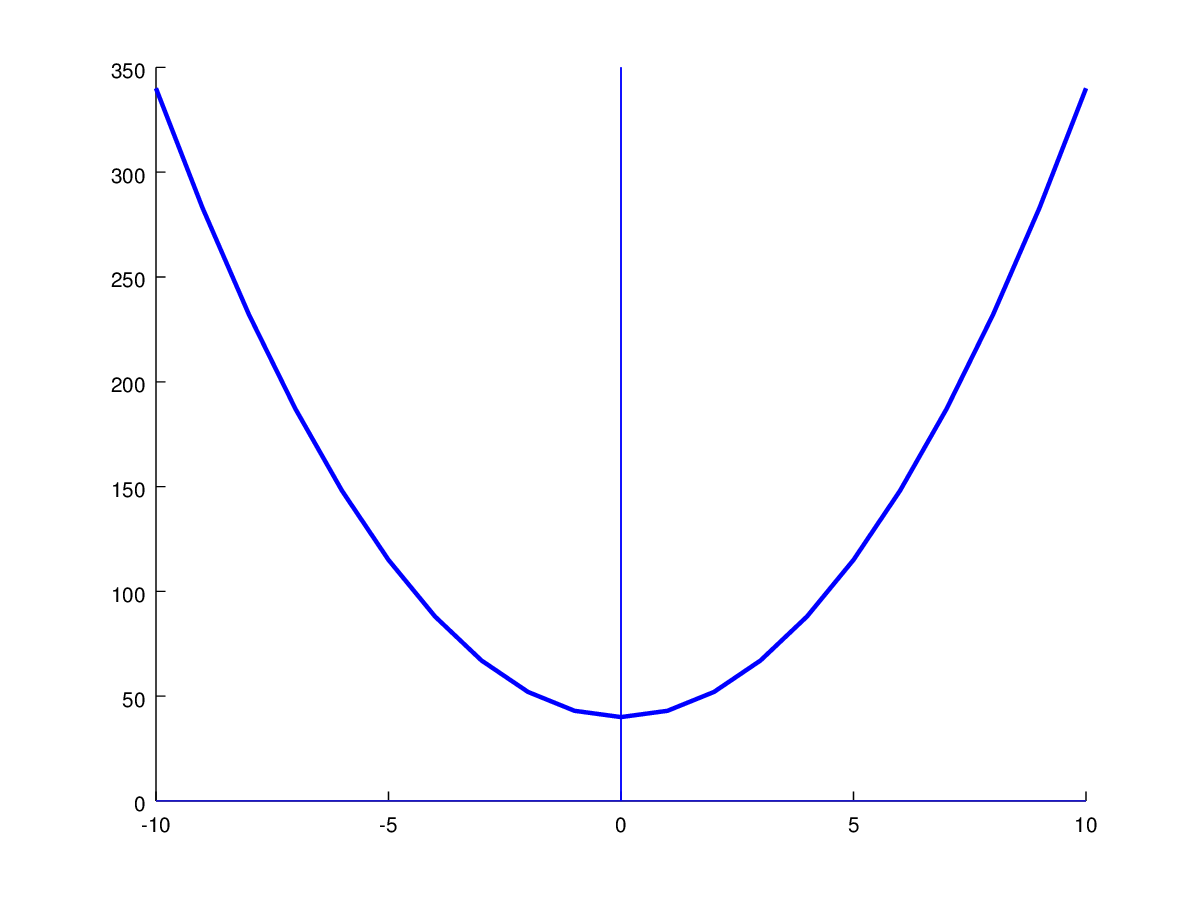
\includegraphics[width=0.8\linewidth]{imgs2/chart7.png}
	\caption{Um exemplo de $\Delta < 0$}
\end{figure}

\newpage

\section{Exercícios}
\begin{enumerate}
	\item Diga se as expressões a seguir são uma função do segundo grau 
		ou não:
	\begin{enumerate}
		\item $f(x) = -3x^2 + x - 34$
		\item $f(x) = \frac{1}{x} - 34 + 3x + 8x^2$
		\item $f(x) = 3x(1 + x^2)$
		\item $f(x) = 4x^2 + 4x - 3 + 4.3x - 12x^2$
		\item $f(x) = 3x + 2x^2$
		\item $f(x) = 5 + 2\sqrt{x}$
		\item $f(x) = 3(1 + x^2) - x$
		\item $f(x) = 1 + 4x$
	\end{enumerate}

	\item Faça uma tabela com os valores em $-10$, $0$ e $10$ para a 
		função $f(x) = 2 + 5x - 3x^2$ e esboce-a no gráfico.

	\item Para as seguintes funções a seguir, diga se elas têm concavidade 
		para cima ou para baixo e esboce-as no gráfico 
		(só precisa esboçar a concavidade corretamente):
	\begin{enumerate}
		\item $f(x) = 4x^2$
		\item $f(x) = 8 - 3x^2$
		\item $f(x) = 6x^2 - 800x$
	\end{enumerate}
\end{enumerate}

\newpage

\section{Respostas aos exercícios}
\begin{enumerate}
	\item 
	\begin{enumerate}
		\item Sim.
		\item Não.
		\item Não. (distribuindo, aparece $x^3$)
		\item Sim.
		\item Sim.
		\item Não.
		\item Sim.
		\item Não.
	\end{enumerate}

	\item 
		\begin{table}[H]
			\centering
			\begin{tabular}{| c | c |}
				\hline
				x & $f(x)$\\
				\hline
				-10 & -348\\
				\hline
				0 & 2\\
				\hline
				10 & -248\\
				\hline
			\end{tabular}
		\end{table}
		Gráfico:
		\begin{figure}[H]
			\centering
			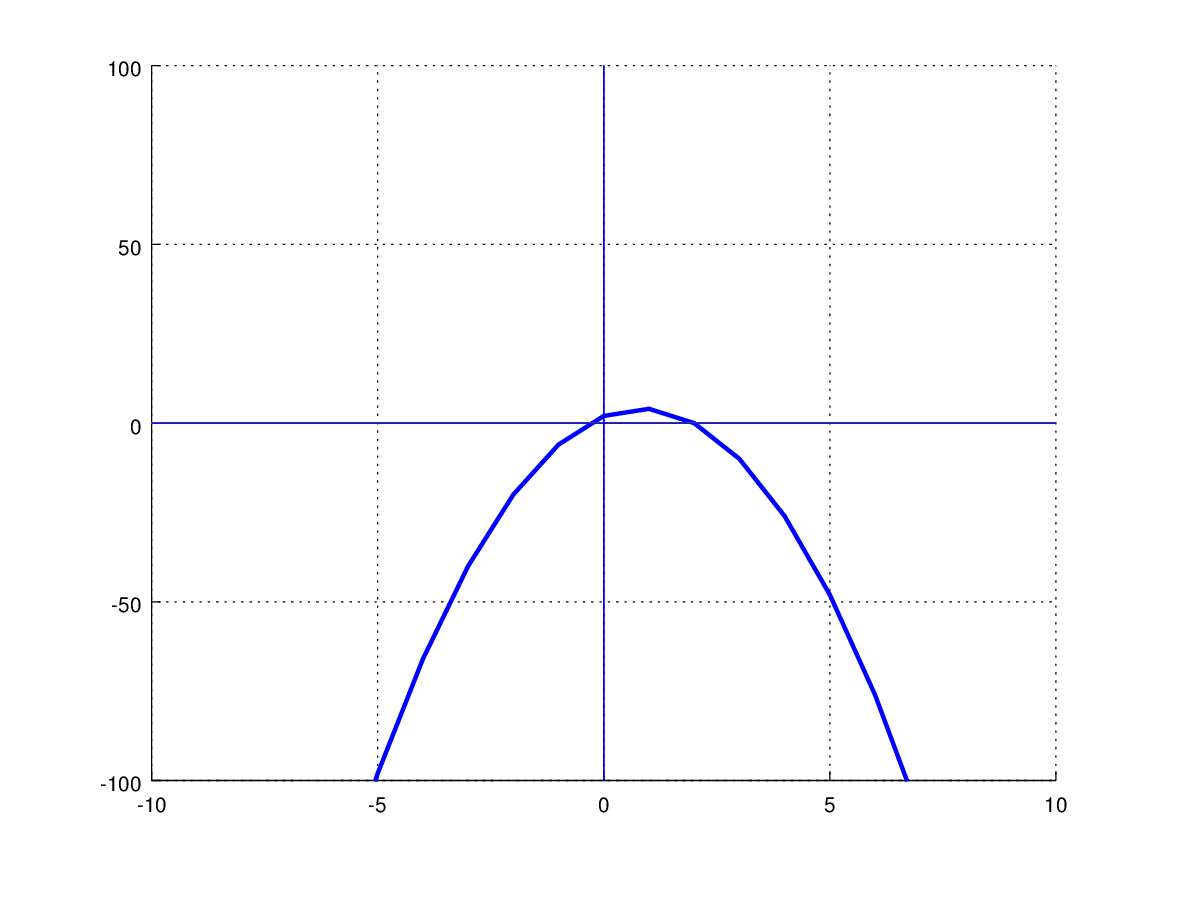
\includegraphics[width=0.8\linewidth]{imgs2/chart8.png}
		\end{figure}
		
	\item 
	\begin{enumerate}
		\item Concavidade para cima.
		\begin{figure}[H]
			\centering
			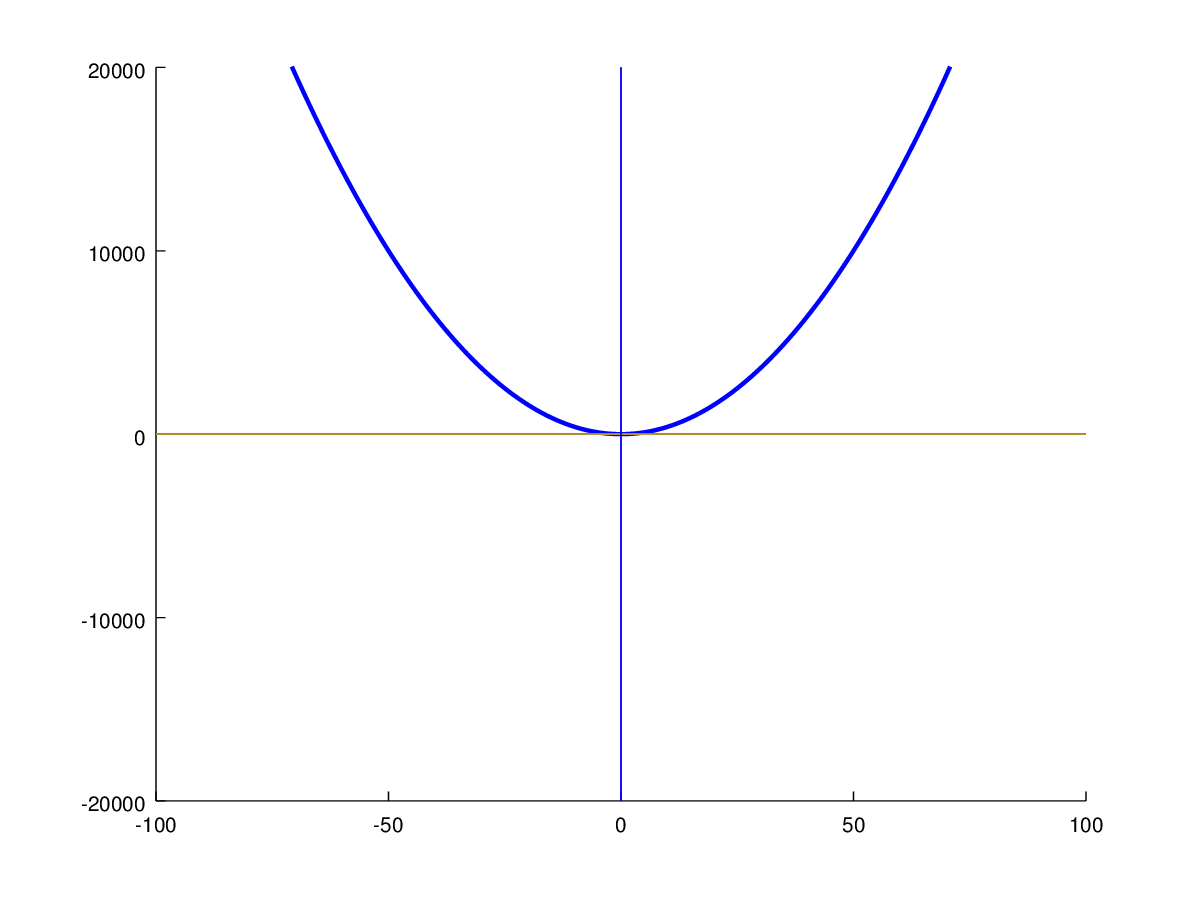
\includegraphics[width=0.8\linewidth]{imgs2/chart9.png}
		\end{figure}
		\item Concavidade para baixo.
		\begin{figure}[H]
			\centering
			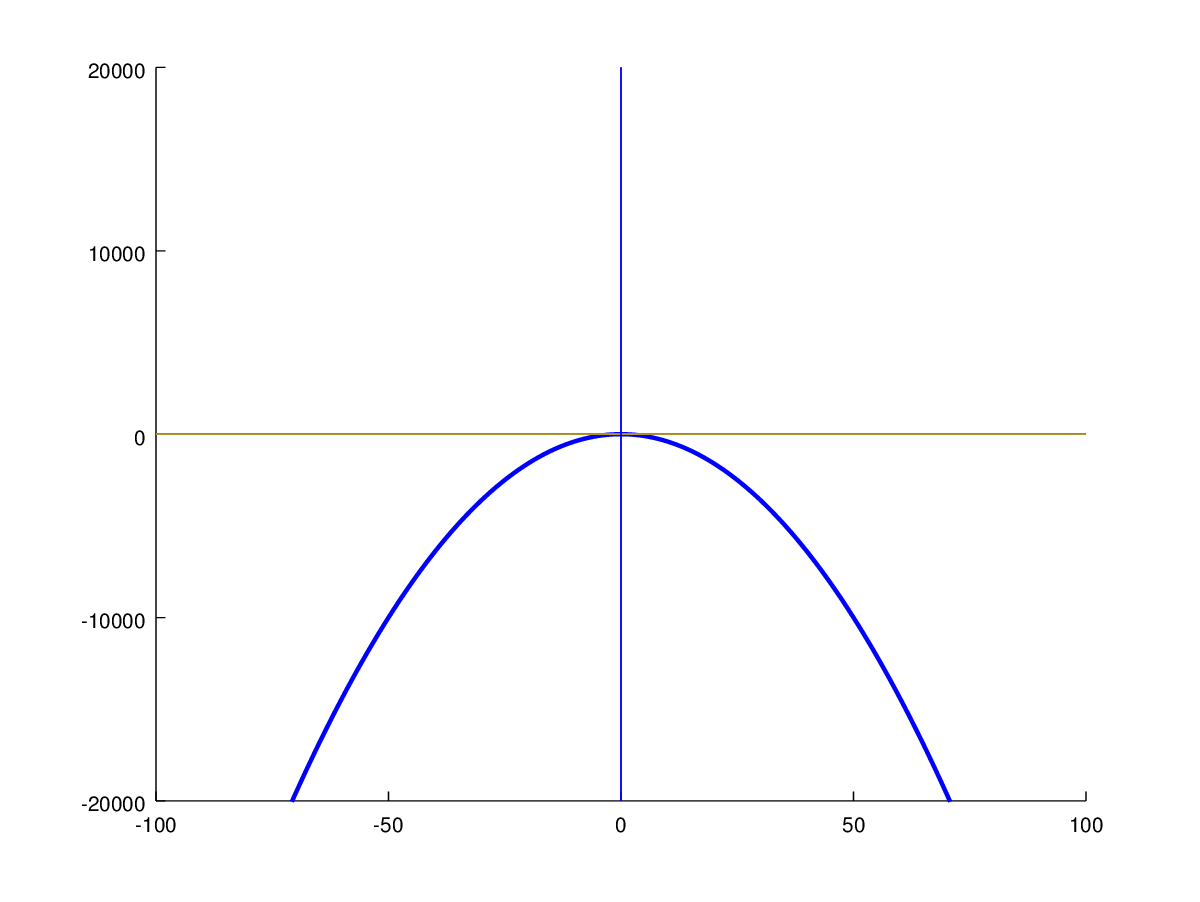
\includegraphics[width=0.8\linewidth]{imgs2/chart10.png}
		\end{figure}
		\item Concavidade para baixo. 
		\begin{figure}[H]
			\centering
			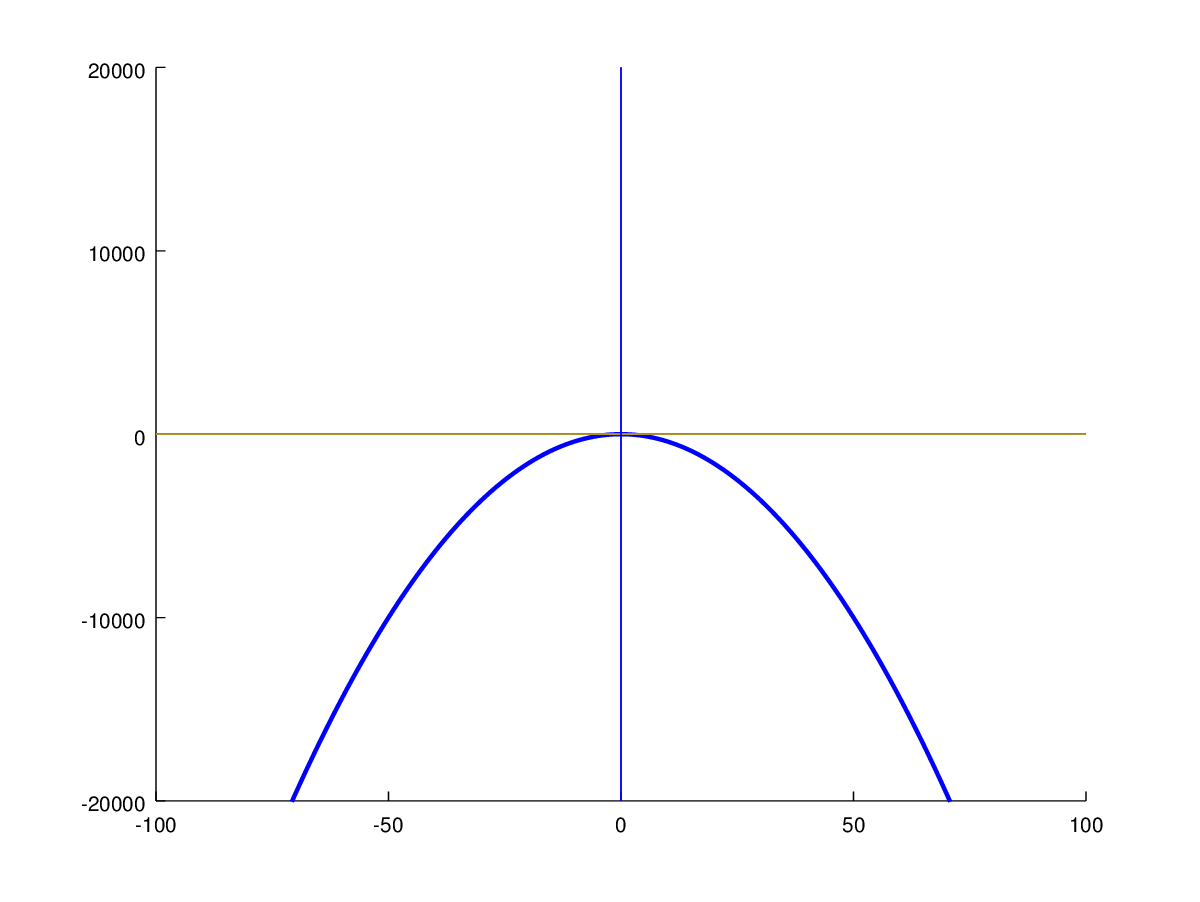
\includegraphics[width=0.8\linewidth]{imgs2/chart10.png}
		\end{figure}
	\end{enumerate}
\end{enumerate}


\end{document}
